% Ausarbeitung der Architektur
\chapter{Architektur von Softwaresystemen}
\label{sec:softwarearchitektur}

Die virtuelle Welt wächst immer schneller und schneller, die Digitalisierung ist mitten im Gange. Schlagzeilen über Industrie 4.0, \ac{IoT}, Cloud, Block Chain, \ac{DevOps}, BigData oder \ac{AI} tauchen immer öfter in den digitalen Nachrichten Welt auf. Viele Unternehmen setzten sich das Ziel, deren Strukturen zu modernisieren, so wie die Unternehmensprozesse zu optimieren. Diese sollen flexibler, schneller und effizienter ablaufen. Doch auch Privatpersonen rüsten stark nach, ein Leben ohne Smartphone ist heutzutage kaum noch vorstellbar. Navigation, Kommunikation, Unterhaltung, Shopping, Banking und vieles mehr damit sind möglich, ein Gerät für alle Fälle. Allein im zweiten Quartal des Jahres 2019 stehen über 4.5 Millionen Anwendungen für sogenannte Smartphones zur Verfügung und es werden täglich immer mehr\autocite[Vgl.][]{appstore}.
%Appfigures. (2019). Anzahl der verfügbaren Apps in den Top App-Stores im 2. Quartal 2019. Statista. Statista GmbH. Zugriff: 26. August 2019. https://de.statista.com/statistik/daten/studie/208599/umfrage/anzahl-der-apps-in-den-top-app-stores/

Der Wandel unter dem Schlagwort \textit{Digitale Transformation} hat natürlich auch gravierende Auswirkungen auf die Systemarchitekturen. Denn die Bauweisen solcher Systeme sollen Zukunftsfähig sein, obwohl dies nicht so einfach ist, schon allein weil heute noch nicht bekannt ist, was morgen neu erscheinen wird. Die Gefahr besteht darin, dass viele der aktuellen \ac{IT}-Systeme in ihrer Existenz bedroht wären, wenn sie keine grundlegende Modularisierung vorweisen könnten. Genau deshalb muss das Ziel der modernen \ac{IT}-Entwickler sein, deren Systemarchitekturen so zu gestalten, dass eine möglichst hohe Modularität und Flexibilität eine Grundlage deren wird\autocite[Vgl.][17\psq]{gmodse}.


Die Modularisierung ermöglicht die Beherrschung der \textit{digitalen Transformation}. Dadurch entstehen Flexibilitätsvorteile, die die ideale Reaktion auf das dynamische Wachstum der Digitalisierung ist. Somit handelt es sich beim Thema Modularisierung um eine der wichtigsten Konzepte der Softwarearchitektur. Die Modularisierung eines \ac{IT}-Systems ist erfüllt, wenn das gesamte \ac{IT}-System in einzelne Komponente zerlegt werden kann. Jede einzelne Komponente ist als abgegrenzter Teil des Systems definiert und übernimmt eine entsprechende Funktionalität des \ac{IT}-Systems. 

Die einzelnen Komponenten sollten möglichst unabhängig voneinander sein und zudem die einfache Ersetzbarkeit durch eine andere Komponente mit denselben Eigenschaften ermöglichen. Auch bei einem Ausfall einer der Komponenten wird das System weiterhin funktionieren, dann eben ohne die Funktionalität der ausgefallenen Komponente.

Die Zerlegung in einzelne Komponenten bieten folgende Vorteile\autocite[Vgl.][3\psq]{gmodse}:
\begin{itemize}
\item Diese können ohne Seiteneffekte und Abstimmungsarbeit weiterentwickelt werden.
\item Diese können unabhängig von Rest dokumentiert und verstanden werden.
\item Diese können an ihren ein- und ausgehenden Schnittstellen isoliert getestet werden.
\item Diese können leicht ausgetauscht werden.
\item Diese sind flexibel an das Wachstum des \ac{IT}-Systems anpassbar.
\item Diese reduzieren die Komplexität des \ac{IT}-Systems.
\end{itemize}

\begin{quote}
\glqq{}Sollte eine Software mit der Zeit irgendwelche Probleme bekommen, sei es beispielsweise mit der Stabilität oder mit der Wartbarkeit, so werden sich diese Probleme, so man auch immer auf Modularisierung geachtet hat, immer nur auf einen Teil des Systems beziehen und niemals auf die gesamte Software. Software ab einer gewissen Größenordnung, die keine erkennbaren Strukturen aufweist, kommt potenziell in existenzielle Bedrohung, sobald sie die ersten Probleme dieser Art aufweist.\grqq{} \footnote{a.a.O., S. 3.}
\end{quote}

Ein ausgezeichnetes Negativbeispiel dafür sind die aktuellen Hochschul-\acp{App}. Diese wurden für jedes System separat Entwickelt und das nur mit genau den Funktionalitäten, die zu dieser Zeit erforderlich waren. Somit hat jedes \ac{IT}-System eine eigene Softwarearchitektur bekommen und die Funktionalitäten wurden für jedes System auf eine andere Art und Weise implementiert. Jedoch sind durch die bereits erwähnte Digitalisierung über die Jahre immer neue Anforderungen an die \ac{IT}-Systeme entstanden. Diese wurden bereits ausführlich in Kapitel \ref{sec:anforderung} beschrieben. Durch die nicht modularisierte Gestaltung der Softwarearchitektur der bestehenden \ac{IT}-Systemen ist die Entwicklung bei einem Punkt angekommen, bei der gemeinsame Erweiterungen oder Änderungen der Anwendungen für alle \ac{IT}-Systeme entweder aufwändig oder sogar nicht möglich sind.
\\
\linebreak
Somit handelt es sich bei der Erstellung einer Softwarearchitektur um eine der wichtigsten Disziplinen in der \ac{IT}-Branche. Zu beachten ist jedoch, dass die Softwarearchitektur nicht nur aus dem Drang nach Modularität besteht, denn es müssen noch viele andere wichtigen Anforderungen und Prinzipien eingehalten werden, um eine zukunftsfähige Softwarearchitektur zu erstellen. Auf diese Anforderungen und Prinzipien wird in den nächsten Kapiteln eingegangen. Außerdem muss berücksichtigt werden, dass nur modulare Softwarearchitekturen in Frage kommen, denn das Ziel dieser Bachelorarbeit ist es, eine erweiterbare, betriebssystemunabhängige Hochschul-\ac{App} zu entwickeln.


\section{Grundlegendes}
Die Realisierung eines jeden Projekts benötigt immer einen ersten Architekturentwurf. Egal welche Industriezweige es betrifft, ob der Bau einer Brücke geplant werden soll, ein Netzwerk umgesetzt werden muss oder eine Anwendung implementiert werden soll, am Anfang steht immer die Architektur. Ein früher Entwurf, der später noch detaillierter beschrieben werden kann, bietet anfangs eine gute Grundlage für vorzeitige Bewertungen und Entscheidungen zur Verteilung der Ressourcen. Außerdem lassen sich oft vorzeitig Probleme erkennen und schneller beheben.
\\
\linebreak
Beim Entwurf einer Anwendung werden die Spezifikationen der einzelnen Funktionalitäten in Komponente zerlegt um die Komplexität weitgehend nach dem Prinzip \textit{teile und herrsche} zu minimieren. Dabei wird der Aufbau der benötigten Teilsysteme, sowie die Festlegung der Verbindungen und Abhängigkeiten der Komponenten untereinander, beschrieben. Jedoch besteht eine Softwarearchitektur nicht nur aus der Anwendung selbst. Stattdessen müssen auch andere Schichten beachtet werden, um einerseits die nicht-funktionalen Anforderungen abzudecken und andererseits die Anpassung an die Umgebung, auf dem die Anwendung später implementiert werden soll, zu gewährleisten. Zudem muss auch auf die nötige Middleware eingegangen werden, die benötigt wird, um mit externen Systemen kommunizieren zu können. Somit ist die Entscheidung des Software-Designs einer der wichtigsten Punkte bei Erstellung einer Anwendung\autocites[Vgl.][]{onlinelexikonsa}[Vgl.][1]{gmodse}.

\section{Nicht-funktionale Anforderungen}
\label{sec:nfa}
Die nicht-funktionale Anforderungen sind meistens die Anforderungen, die nicht explizit vom Auftraggeber erwähnt werden, sondern die, die sich eher automatisch aus den Vorgaben ergeben oder die man bei aktueller Software als selbstverständlich sieht. Die meisten solcher Anforderungen sind in Abbildung \ref{fig:anforderungen} zu sehen.

\begin{figure}[H]
\centering
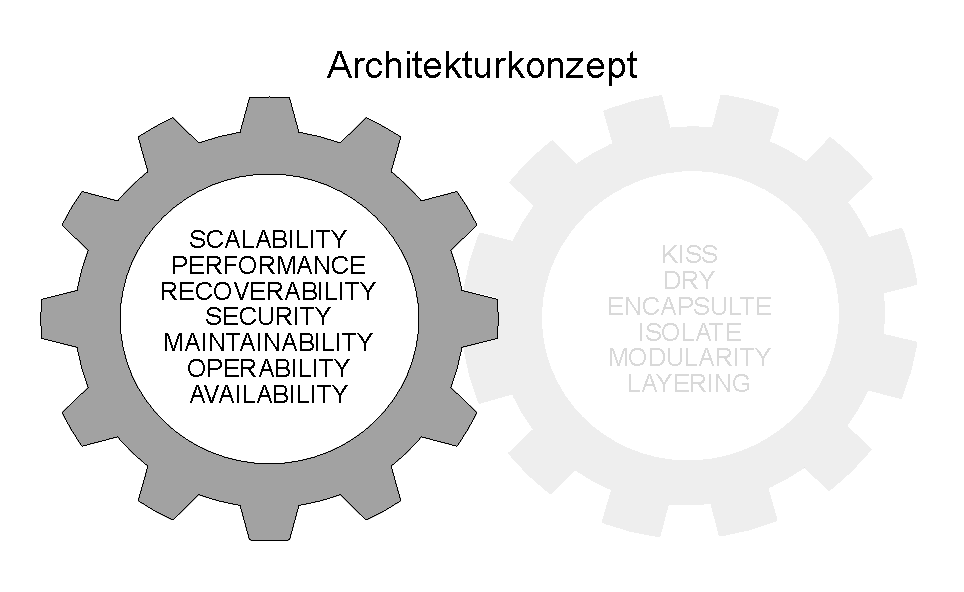
\includegraphics[width=\pictureWidth cm]{Bilder/Sonstiges/Anforderungen_Prinzipien-Transparent.pdf}
\caption{Allgemeine Anforderungen an eine Architektur\label{fig:anforderungen}\protect\footnotemark}
\end{figure}
\footnotetext{Brysiuk, Lehmann (2019)}

Es ist bei einem Softwareentwurf immer wichtig, sich über alle nicht-funktionalen Anforderungen Gedanken zu machen, denn diese bilden den Grundbaustein für eine erfolgreiche und zukunftsfähige Anwendung. Dadurch können spätere Mängel leichter behoben werden, neue Anforderungen schneller umgesetzt werden und die Anwendung an das Wachstum der Hochschule angepasst werden.

\section{Prinzipien}
\label{sec:prinzipien}

Ein weiterer wichtiger Punkt ist die Beachtung von Prinzipien beim Softwareentwurf. Diese werden bei den nicht-funktionalen Anforderungen aus Abbildung \ref{fig:anforderungen} im Architekturkonzept ergänzt. Das Resultat in Abbildung \ref{fig:prinzip} bietet eine Basis zur Vorgehensweise bei der Entwicklung eines Softwareentwurfs.

\begin{figure}[H]
\centering
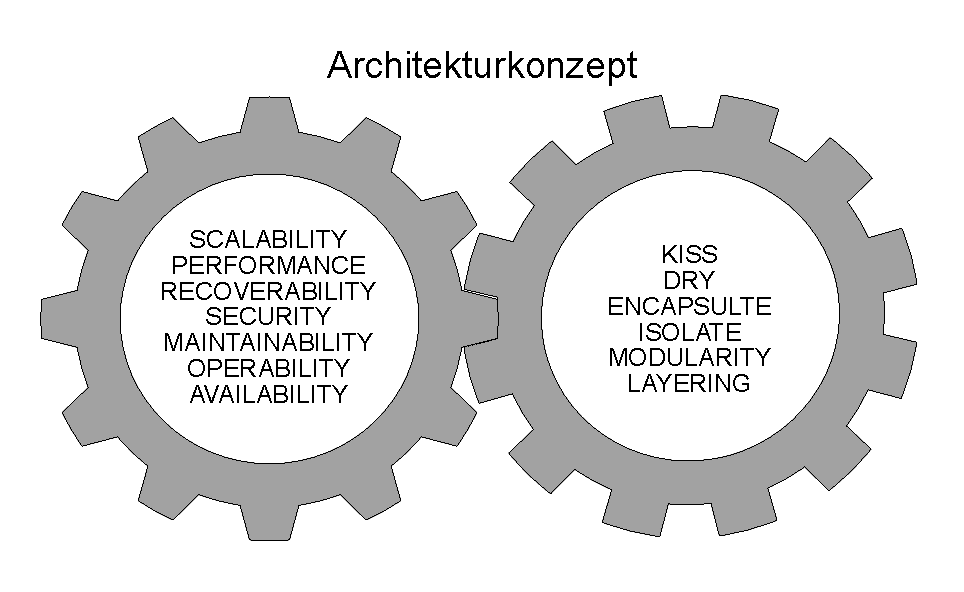
\includegraphics[width=\pictureWidth cm]{Bilder/Sonstiges/Anforderungen_Prinzipien.pdf}
\caption{Allgemeine Prinzipien einer Architektur\label{fig:prinzip}\protect\footnotemark}
\end{figure}
\footnotetext{Brysiuk, Lehmann (2019)}

Die nicht-funktionalen Anforderungen sind im allgemeinen selbsterklärend, deshalb wird nicht weiter auf sie eingegangen. Jedoch bestehen die Prinzipien des Softwareentwurfs aus weniger selbsterklärenden Begriffen und Akronymen, weshalb diese im folgenden genauer erläutert werden.

\subsection*{KISS - Keep it Simple and Stupid}

Bereits im 20. Jahrhundert hat der amerikanische Flugzeugkonstrukteur Clarence Leonard (Kelly) Johnson das \ac{KISS}-Prinzip erstmals erwähnt und treffend beschrieben:
\begin{quote}
\glqq{}Reduce reports and other paperwork to a minimum.\grqq{} \autocite[][231]{biography}
\end{quote}

Die Idee dahinter ist, dass die Gestaltung der Maßnahmen oder Entscheidungen so wenig wie möglich Komplexität beinhalten, jedoch sollen die Ergebnisse die erwarteten Anforderungen erfüllen und dazu flexibel genug sein, um Änderungen vorzunehmen. Also soll die Umsetzung einfach, schnell, verständlich, logisch, begreifbar und passend an die Anforderungen und nicht auf die Möglichkeiten sein. Bei einer Softwarearchitektur darf bei der Einhaltung des \ac{KISS}-Prinzips nicht auf die angemessene Modularisierung verzichtet werden\autocite[Vgl.][19]{gmodse}.

Häufig wird beim Konzeptionieren versucht von Anfang an auf alle möglichen Variationen der Anforderungen einzugehen. Dies umfasst auch die Anforderungen, die noch nicht gestellt wurden, von denen man allerdings ausgeht, as sie im Verlauf des Projektes noch vom Auftraggeber ergänzt werden. Das Ziel davon ist es, in der Zukunft den zusätzlichen Aufwand für die Implementierung zu sparen. Das Problem dabei ist, dass die Wahrscheinlichkeit ziemlich gering ist, dass solche zusätzliche Funktionalitäten tatsächlich noch benötigt werden. Das führt letztendlich zu einer komplexeren Anwendung, deren Flexibilität auf ein Minimum reduziert wird. Dies wird zusätzlich dadurch unterstützt, dass eine Anforderung sich während des Entwicklungsprozesses ändert, da der Auftraggeber oft nicht mehr zufrieden mit der ursprünglichen Lösung ist\footnote{a.a.O., S. 19 f.}.
\\
\linebreak

\begingroup

Folgende Formel zur Berechnung des Nutzen eines Mehrwerts ~$N_{mehrwert}$ kann dazu dienen, besser abschätzen zu können, ob ein gewünschter Mehrwert tatsächlich vorher berücksichtigt werden soll\footnote{a.a.O., S. 20.}:
\\
\linebreak

\begin{dmath}
N_{mehrwert} = (A_{nach} * P_{gebrauch}) - A_{vor}
\end{dmath}

\par
\begingroup
\leftskip=2cm
\rightskip=2cm
\noindent \textit{wobei \\~$A_{vor} =$ Aufwand eines Features bei der Planung von Anfang an\\~$A_{nach} =$ Aufwand eines Features bei späterer Aufnahme\\~$P_{gebrauch} =$ Wahrscheinlichkeit, dass ein Feature später benötigt wird}
\par
\endgroup
\endgroup

\subsection*{DRY - Dont't Repeat Yourself}

<Durch generische Programmierung können Code-Duplikate vermieden werden und wiederholende Algorithmen an mehreren Stellen wiederverwendet werden. Die Idee ist es also beim DRY-Prinzip, die Redundanzen von Programmstellen zu reduzieren , beziehungsweise sie komplett zu vermeiden. Hier ist aber Vorsicht geboten, denn die nicht-funktionalen Anforderungen wie Verfügbarkeit oder Wartbarkeit haben eine höhere Priorität. Man soll alle Prinzipien und Anforderungen auswerten und sogar priorisieren, um eine ausgewogenen Softwarearchitektur erstellen zu können\autocite[Vgl.][21]{gmodse}.

\subsection*{Encapsulation - Prinzip der Kapselung}
Das Konzept des \textit{Information Hidings} wurde bereits im Jahr 1972 von David Parnas vorgestellt:

\begin{quote}
\glqq{}The second decomposition was made using \grqq{}information hiding\grqq{} as a criterion. The modules no
longer correspond to steps in the processing. The line
storage module, for example, is used in almost every
action by the system. Alphabetization may or may not
correspond to a phase in the processing according to
the method used. Similarly, circular shift might, in some
circumstances, not make any table at all but calculate
each character as demanded. Every module in the
second decomposition is characterized by its knowledge
of a design decision which it hides from all others. Its
interface or definition was chosen to reveal as little as
possible about its inner workings.\grqq{} \footcite[][1056]{parmas}
\end{quote}

Der Zweck besteht darin eine Art Geheimnisprinzip zu erstellen, um bestimmte Stellen zu schützen, ob für die Zugriffsberechtigungen oder für die Sicherung der Integrität der Daten. Es werden Komponenten verborgen und eine Schnittstelle für einen öffentlichen Zugriff definiert, somit hat eine Änderung oder der Austausch einer Komponente keine Auswirkung nach außen. Außerdem wird die Robustheit der Anwendung durch die erhöhte Begrenzung der Abhängigkeiten der Komponenten gestärkt\autocite[Vgl.][21\psq]{gmodse}.

\subsection*{Lose Kopplung}
l
\ac{IT}-Systeme bestehen meist aus mehreren Bausteinen, Komponenten und Subsystemen. Diese werden immer zwangsläufig Abhängigkeiten untereinander bilden, da einfach das ganze \ac{IT}-System nicht völlig isoliert werden kann. Die Idee der losen Kopplung ist es, die Verbindungen der einzelnen Bausteine untereinander zu verringern, sowohl auf der Hardware-, als auch auf der Softwareebene. Bei den Verbindungen sollen folgende Punkte berücksichtigt werden\autocite[Vgl.][25\psqq]{gmodse}:

\begin{itemize}
\item Laufzeitumgebungen
\item Ausführungsort
\item Verwendete Technologien
\item Ausführungszeit
\item Daten und Formate bei der Kommunikation
\end{itemize}

\subsection*{Separation Of Concerns}

Auf das Prinzip \textit{Seperation Of Concerns}, zu Deutsch etwa \textit{Trennung der Angelegenheiten}, wurde im Verlauf den gesamten Kapitels immer wieder aufmerksam gemacht und auf dessen Wichtigkeit hingewiesen. \textit{Separation of Concerns} ist das Prinzip der Modularität, welches bereits ausführlich am Anfang des Kapitels \ref{sec:softwarearchitektur} beschrieben wurde.

\subsection*{Layering - Schichtenarchitektur\label{sec:layering}}
Wie bereits in Prinzip der Modularität beschrieben wurde, ist es wichtig beim Entwurf eines \ac{IT}-Systems dieses in einzelne Komponente und Module zu zerlegen. Dabei bilden die Komponenten in ihrem Zusammenspiel auf einer Ebene verschiedene Schichten. Dieser Schichten sind nach Funktionalität getrennt. Beispielhaft ist das in der Abbildung \ref{fig:schichten} dargestellt. Das System besteht aus vier verschiedenen Schichten die wiederum einzelne Komponenten enthalten\footnote{Vgl. a.a.0., S. 31 ff.}.

\begin{figure}[H]
\centering
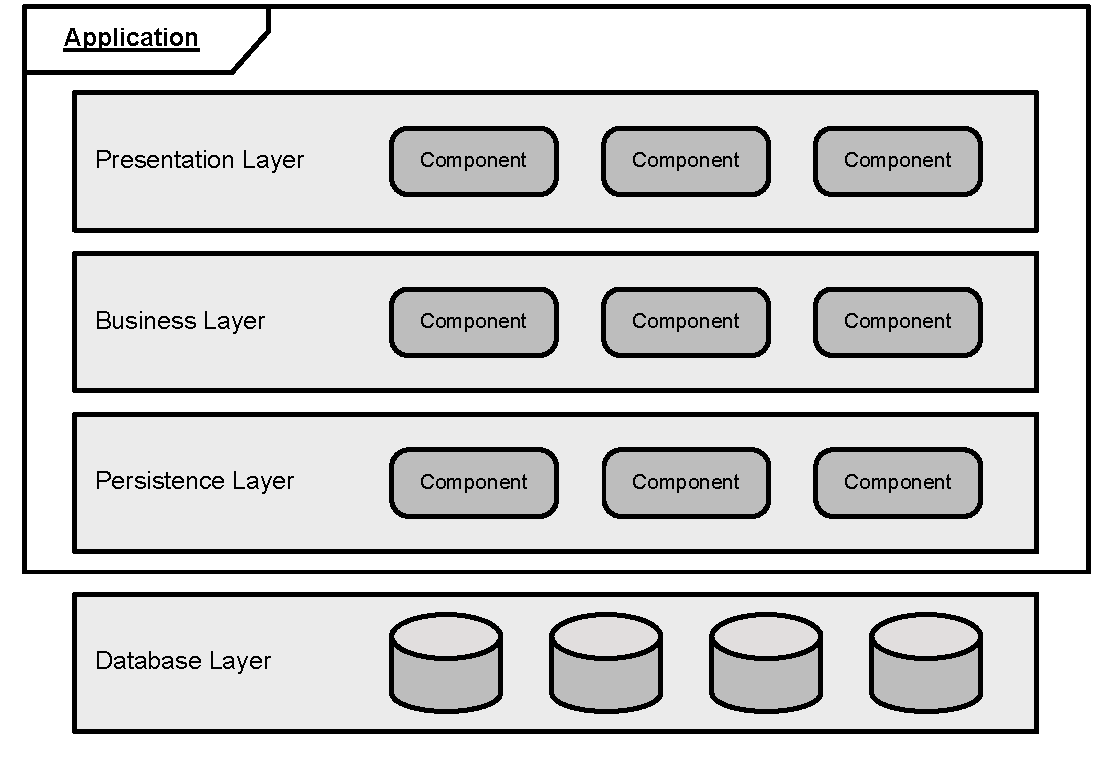
\includegraphics[width=\pictureWidth cm]{Bilder/Architektur/Schichtenarchitektur.pdf}
\caption{Schichtenarchitektur\label{fig:schichten}\protect\footnotemark}
\end{figure}
\footnotetext{Vgl. Dowalil(2018), S. 31 ff.}

Für Entwickler werden große Projekte durch die Einhaltung des \textit{Layerings} deutlich beherrschbarer. Ähnlich wie unser Gehirn solche Zusammenhalte verarbeitet wird das große Ganze in Schichten unterteilt, die sich in Funktionalitäten trennen. Die einzelnen Schichten werden dann wieder in Komponenten zerlegt, bis eine Komponente klein genug ist um sie detailliert zu verstehen. So muss man sich am Ende nur einen Überblick über das Gesamtbild verschaffen\footnote{Vgl. a.a.O., S. 36.}.

\section{Fazit\label{sec:archfazit}}
Die Verbreitung der verteilten Programme, im Englischen \textit{Distributed \acp{App}}, hat sich in den vergangenen Jahren schnell weiterentwickelt. Diese Anwendungen laufen nicht auf einem einzelnen lokalen Rechner, sondern werden auf mehrere unabhängige Module verteilt, die wiederum auf mehreren unterschiedlichen Servern im Netzwerk verteilt sein können. Somit stellen verteilte Anwendungen eine Art verteiltes - beziehungsweise vernetztes - System dar\autocite[Vgl.][3\psq]{verteiltesys}. 
\\
\linebreak
Ein Beispiel hierfür sind Cloud Computing Systeme, diese bauen auf der Softwarearchitektur von verteilten Systemen auf. In Abbildung \ref{fig:cloud_statistic} ist eine Statistik abgebildet, in der das Wachstum für die Nutzung von Cloud Computing Systemen in deutschen Unternehmen in den Jahren 2011 bis 2018 zu sehen. Man erkennt, dass bereits im Jahr 2018 73\% der befragten Unternehmen Cloud Computing Systeme benutzten. Weitere 19\% überlegten oder planten bereits solche Systeme zu nutzen\autocite{cloudstatista}.

\begin{figure}[H]
\centering
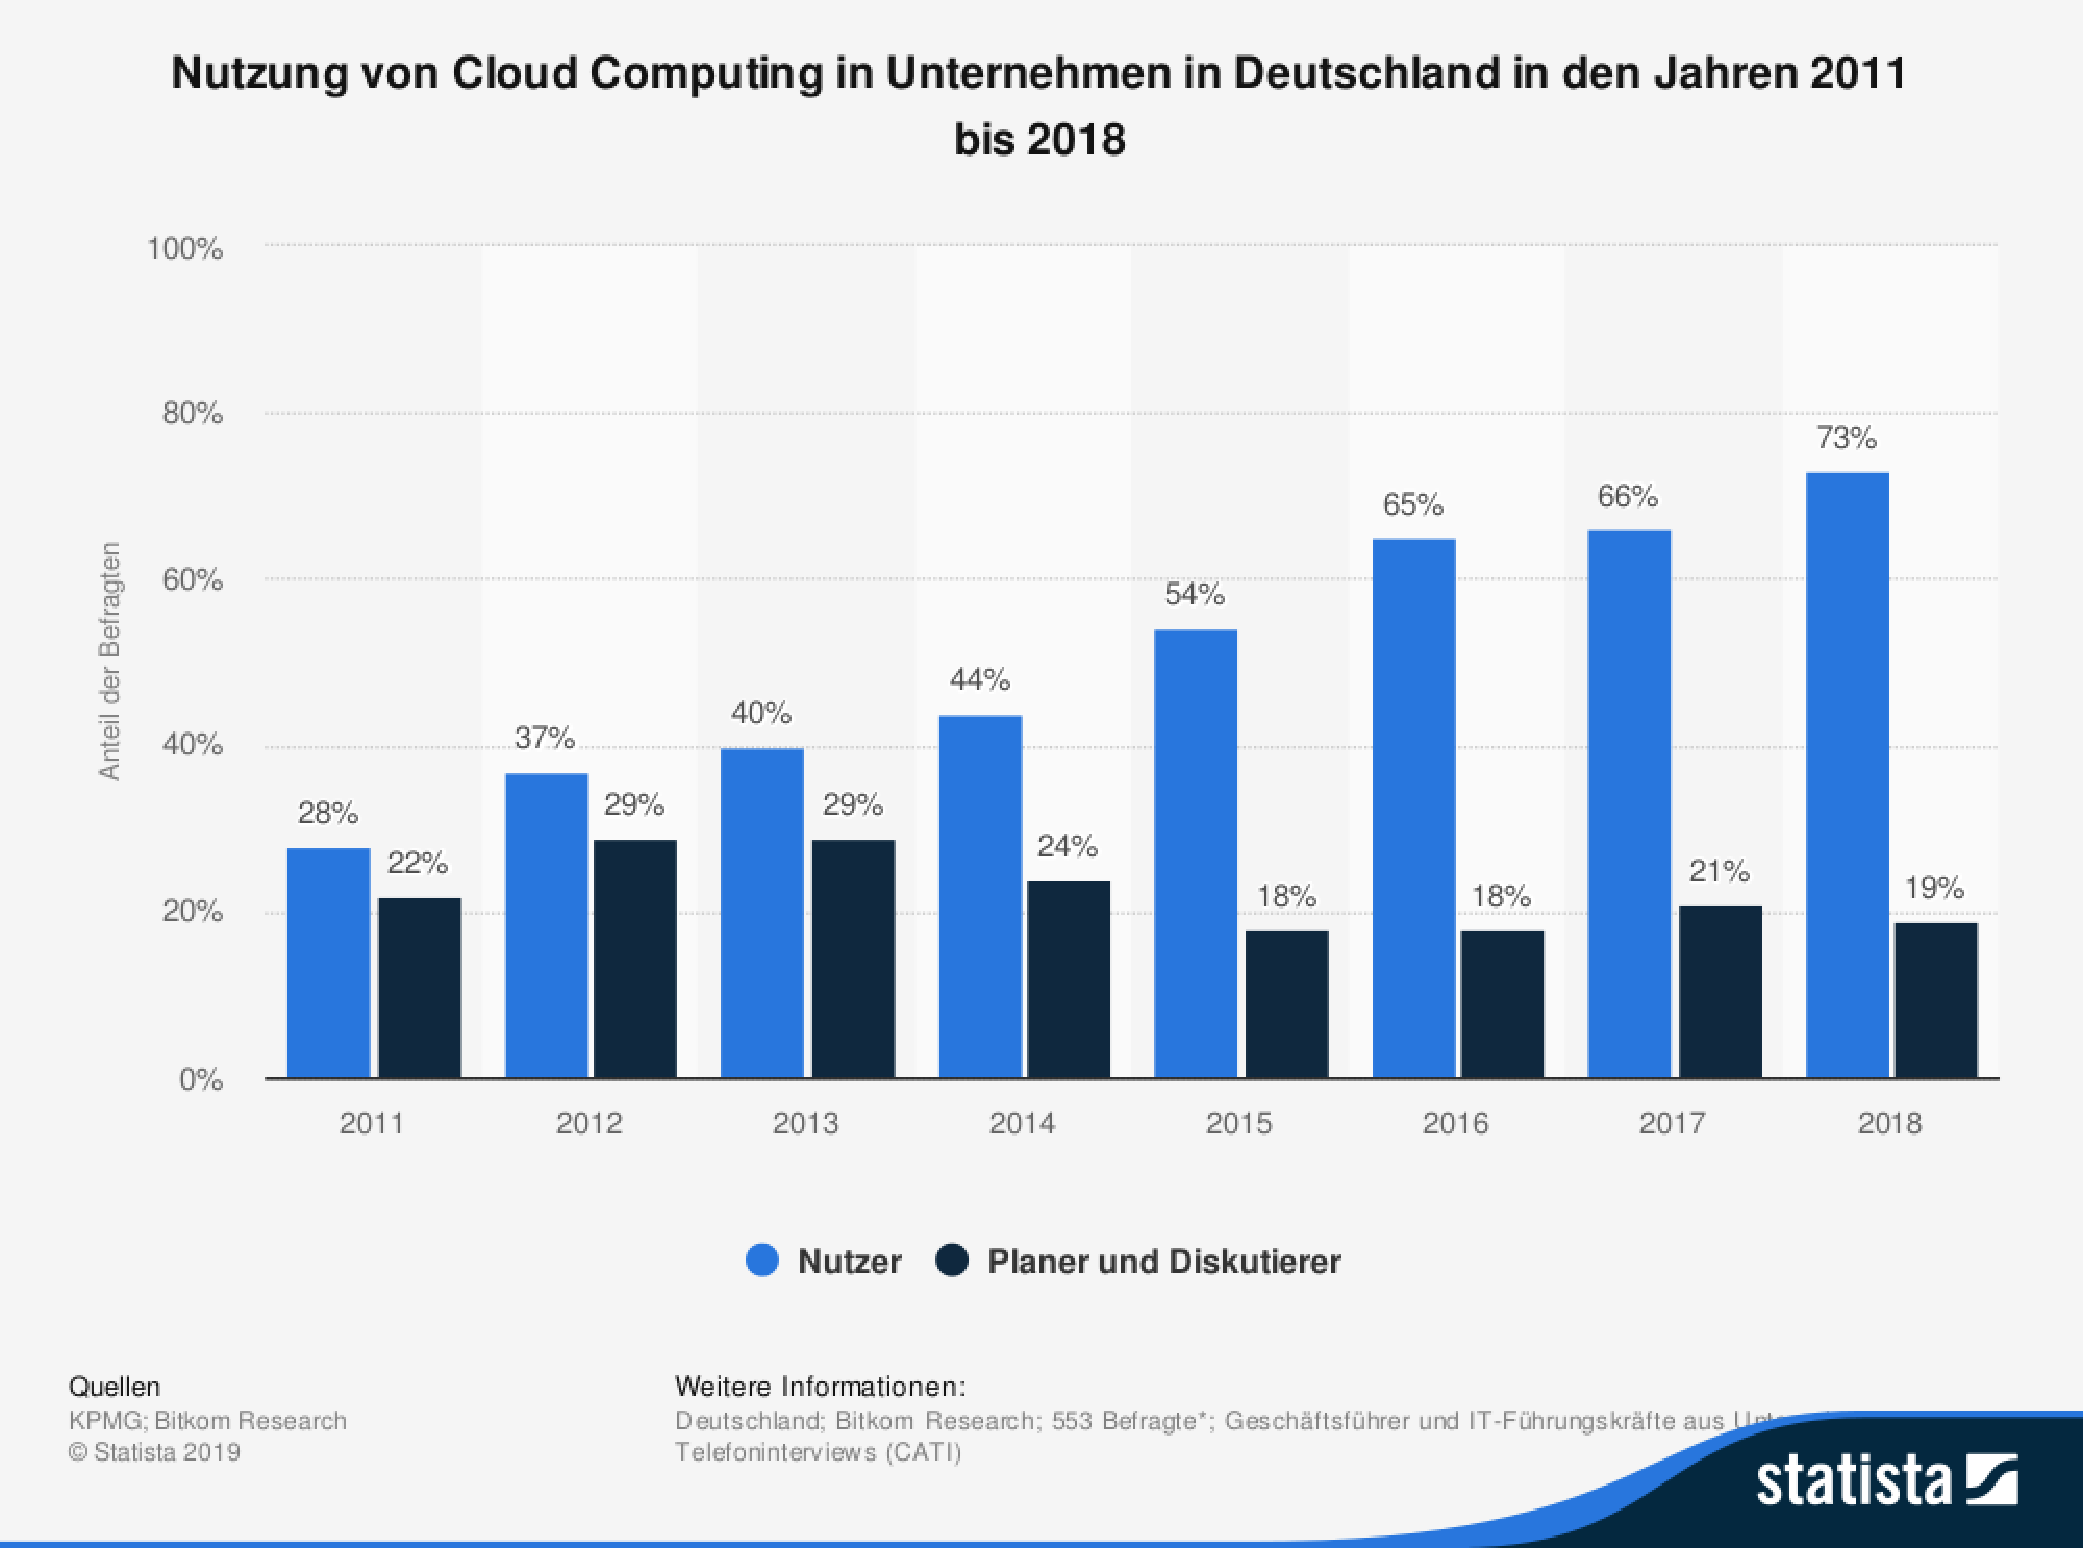
\includegraphics[width=\pictureWidth cm]{Bilder/Statistik/Statista_Cloud_Computing.pdf}
\caption{Nutzung von Cloud Computing\label{fig:cloud_statistic}\protect\footnotemark}
\end{figure}
\footnotetext{ebd.}
% Bitkom, Nutzung von Cloud Computing in Unternehmen in Deutschland in den Jahren 2011 bis 2018 Statista, https://de.statista.com/statistik/daten/studie/177484/umfrage/einsatz-von-cloud-computing-in-deutschen-unternehmen-2011/ (letzter Besuch 14. August 2019)

Wie bereits erwähnt setzen sich verteilte Systeme aus mehreren unabhängigen Modulen zusammen, die auf unterschiedlichen Servern implementiert sind. Durch die Kopplung der Module entsteht ein vollständiges System, welches eine räumliche Trennung über weite geografische Distanzen ermöglicht. Dies ermöglicht einen parallelen und effizienten Zugriff, in unserem Fall zum Beispiel auf Stundenplan- und Mensadaten, denn die Abfragen würden von zwei unterschiedlichen Modulen auf verschiedenen Servern bearbeitet werden. Einen weiterer Vorteil bei dieser Herangehensweise ist der Lastausgleich. Durch eine Modularisierung der Funktionalitäten und der Verteilung dieser auf mehreren Servern, kann die Verarbeitungslast eines zentralen Servers auf mehrere Instanzen verteilt werden, um eine einseitige Auslastungen zu vermeiden. Außerdem wird ein hohes Maß an Fehlertoleranz, Ausfallsicherheit, Skalierbarkeit und Verfügbarkeit auf der Basis verteilter Systeme gewährleistet\autocite[Vgl.][5\psq]{verteiltesys}.

Ausgehend von den bisherig beschriebenen Anforderungen und Prinzipien an die Softwarearchitektur, sowie der Wichtigkeit von Modularisierung und den Anforderungen aus Kapitel \ref{sec:anforderung}, bieten verteilte Systeme eine gute Voraussetzungen für die Architekturkonzepte der Hochschul-\ac{App}. Dabei bieten diese in sich verschiedene Umsetzungen der Systemarchitektur, die teilweise aufeinander aufbauen\footcite[Vgl.][13\psq]{verteiltesys}:
\begin{itemize}
\item Client-Server-Modell
\item Objektorientiertes Modell
\item Komponenten basiertes Modell
\item Dienst orientiertes Modell
\end{itemize}
Verteilte Anwendungen basieren meist auf dem Dienst orientierten Modell, welches auch unter dem Begriff der \textit{Service-orientierten} Architektur im Zusammenhang mit Webservices bekannt ist\footnote{ebd.}.
Somit sind Webservices ein guter Ansatz für die konkrete Implementierung der verteilten Anwendung und der Grundbaustein für die Hochschul-\ac{App}.
